\documentclass[8pt]{beamer}
\usepackage[nobglogo]{beamerthemedmi-owled}
\usepackage[utf8x]{inputenc}
\usepackage{default}
\usepackage{url}
\usepackage{verbatim}
\usepackage{graphicx}
\usepackage{mathrsfs}
% \usepackage{dl}
% \usepackage{mls}
%\usepackage{listings}


\mode<presentation>
{
  \usetheme{dmi-owled}
  %\usetheme{Warsaw}
  % or ...

  \setbeamercovered{transparent}
  % or whatever (possibly just delete it)
}

\title{Introduzione agli Open Data - Seconda Parte}

\author{Cristiano Longo\\ 
{\small{longo@dmi.unict.it}}}



\date{Universit\`a di Catania, 20 Maggio 2015}
\newcommand{\urlsingle}[1]{{\small {\center {\url{#1}}}}}
\begin{document}
\maketitle
\setcounter{tocdepth}{1}

\section{Riepilogo}


\begin{frame}
\frametitle{Riepilogo}

\begin{quote}
Open means anyone can freely access, use, modify, and share for any purpose (subject, at most, to requirements that preserve provenance and openness).\footnote{\url{http://opendefinition.org}} 
\end{quote}

da \emph{Open Knowledge Foundation: The Open Definition}
\vspace{\baselineskip}

\uncover<2->{
Per rendere effettiva questa definizione \`e necessario prendere in considerazione
diversi aspetti.
\vspace{\baselineskip}

\begin{itemize}[<+->]
 \item \emph{Tecnici} 
 \begin{itemize}
  \item il dato deve essere \emph{liberamente} ottenibile (protocolli e punti di accesso su internet),
  \item semplice da trovare (cataloghi di metadati),
  \item \emph{riusabile} (formati aperti: csv, xml, rdf, odt, ods, \ldots),
  \item modificabile (sorgenti aperti, \emph{raw data}).
 \end{itemize}
 \item \emph{Legali} 
 \begin{itemize}
  \item il dato deve fornito con \emph{licenze aperte} (CC0, CC-BY, CC-BY-SA),
  \item l'apertura non deve violare altre norme (privacy, segreto di stato).
 \end{itemize}
 \item \emph{Sociali} - l'attivit\`a di apertura deve essere adeguatamente pubblicizzata
 presso la cittadinanza e i potenziali \emph{stakeholder}.
\end{itemize}
}
\end{frame}


\begin{frame}
\frametitle{Riepilogo - Ricadute}
Alcune ricadute dell'apertura dei dati:
\vspace{\baselineskip}

\begin{itemize} [<+->]
 \item Economici
 \begin{itemize}
  \item redazione di business plan (vedi l'articolo sui flussi turistici\footnote{\url{http://opendatasicilia.it/2015/05/13/flussi-turistici-e-fruizione-dei-beni-culturali-catania-dal-2012-al-2013/}}),
  \item creazione di nuove imprese basate sui dati (vedi ad esempio \emph{Open Data 500}\footnote{\url{http://www.opendata500.com/us/list/}});
 \end{itemize}
 \item realizzazione di nuovi servizi per i cittadini (vedi ad esempio PETRUSINO,\footnote{\url{http://petrusino.opendatasicilia.it/}}
 ConfiscatiBene,\footnote{\url{http://www.confiscatibene.it/it}} Ordnance Survey,\footnote{\url{https://www.ordnancesurvey.co.uk/innovate/showcase}} Europeana);\footnote{\url{http://labs.europeana.eu/apps}}
 \item trasparenza (vedi ad esempio \url{soldipubblici.it} oppure \url{http://parlamento17.openpolis.it/});
 \item governo partecipato (uno strumento ad esempio è \url{http://www.normattiva.it/}).
\end{itemize}
\end{frame}

\begin{frame}
\frametitle{Esempi}
Alcune esempi di pubbliche amministrazioni che hanno pubblicato i dati, ad esempio
\vspace{\baselineskip}

\begin{itemize} [<+->]
 \item Centrali
 \begin{itemize}
  \item Camera (\url{http://dati.camera.it/}) e Senato (\url{http://dati.senato.it/}) della Repubblica Italiana,
  \item ISTAT (\url{http://dati.istat.it/}),  
  \item Ministero per i Beni e le Attivit\`a Culturali e Turismo (\url{http://www.beniculturali.it/mibac/export/MiBAC/sito-MiBAC/MenuPrincipale/Trasparenza/Open-Data/index.html}, \url{http://www.beniculturali.it/mibac/opencms/MiBAC/sito-MiBAC/MenuPrincipale/LuoghiDellaCultura/Ricerca/index.html});  
 \end{itemize}
 \item Regioni
 \begin{itemize}
  \item Emilia Romagna (\url{http://dati.emilia-romagna.it}),
  \item Lombardia (\url{https://www.dati.lombardia.it}), 
  \item Piemonte (\url{http://www.dati.piemonte.it}), 
  \item Puglia (\url{www.dati.puglia.it}),
  \item Toscana (\url{http://dati.toscana.it}), 
  \item Umbria (\url{http://dati.umbria.it});
 \end{itemize}
 \item Provincie - Provincia Autonoma di Trento e Bolzano (\url{http://dati.trentino.it});
 \item Comuni
 \begin{itemize}
  \item Catania (\url{http://opendata.comune.catania.gov.it}),
  \item Palermo (\url{http://www.comune.palermo.it/opendata_menus.php}),
  \item Matera (\url{http://dati.comune.matera.it}).
 \end{itemize}
\end{itemize}
\end{frame}

\begin{frame}
\frametitle{Strumenti}

Alcuni strumenti per l'utilizzo degli Open Data sono:
\vspace{\baselineskip}

\begin{itemize}
 \item Data Wrapper\footnote{\url{https://datawrapper.de/}} permette di realizzare diagrammi; 
 \item MapBox\footnote{\url{https://www.mapbox.com}} e CartoDB\footnote{\url{https://cartodb.com}} per le mappe;
 \item TABLEAUX e OpenRefine.
\end{itemize}

\end{frame}

\section{Metadati}

\begin{frame}
  \frametitle{Metadati}
  L'aggiunta di \emph{metadati} associati ai daset o ai dati garantisce una maggiore
  \emph{raggiunggibilit\'a} dei dati di interesse da parte degli utenti. Ad esempio
  favorisce l'indicizzazione da parte de motori di ricerca.
  \vspace{\baselineskip}
  
  Questa pratica pu\`o avere anche altre importanti funzioni:
  \begin{itemize}[<+->]
   \item \emph{titolarit\`a} - chi ha prodotto il dato e chi lo mantiene;
   \item \emph{tempestivit\`a} - quale \`e la frequenza di aggiornamento dei dati, se il dato pu\`o essere
   considerato ancora attendibile e per quanto tempo ancora;
   \item \emph{provenienza} - come \`e stato formato il dato ed eventualmente dalla combinazione ed elaborazione
   di quali dataset \emph{primari} \`e stato derivato o importato. 
  \end{itemize}

\uncover<4->{
  Nelle Linee Guida AgID vengono presentate alcune tipologie di metadati \emph{obbligatori} e
  altre di metadati \emph{consigliati}. I metadati obbligatori si suddividono a loro volta in 
  metadati \emph{universalmente} obbligatori, che devono essere 
  sempre presenti, e metadati che sono richiesti solo al in presenza di particolari condizioni.
  \vspace{\baselineskip}
}  

\end{frame}

\begin{frame}
  \frametitle{Metadati Universalmente Obbligatori}

  Riportiamo i metadati sempre obbligatori.
  
  \begin{figure}
    \begin{itemize}[<+->]
      \item \tt{publisher} - soggetto che pubblica il dataset. Spesso coincide con \tt{creator}.
      \item \tt{creator} - soggetto che ha prodotto il dataset.
      \item \tt{rightsHolder} - indica il soggetto o l’organizzazione che detiene e gestisce i diritti sul dataset.
      \item \tt{title} - il titolo del dataset.
      \item \tt{description} - una descrizione in linguaggio naturale del dataset.
      \item \tt{modified} - la data di ultimo aggiornamento.
      \item \tt{accrualPeriodicity} - frequenza di aggiornamento dei dati.
      \item \tt{license} - indica la licenza utilizzata.
      \item \tt{keyword} - parole chiave, separate da virgole, che descrivono il dataset.
    \end{itemize}
    \caption{Metadati Obbligatori}
  \end{figure}
\end{frame}

\begin{frame}
  \frametitle{Metadati Condizionatamente Obbligatori}

  Riportiamo i metadati sempre obbligatori solo in particolari condizioni.
  
  \begin{figure}
    \begin{itemize}[<+->]
    \item \tt{identifier} - solo in caso di LOD, URI che identifica il dataset universalmente.
    \item \tt{spatial} - se i dati hanno significato solo all'interno di una determinata copertura spaziale. 
    \item \tt{temporal} - se i dati hanno significato solo all'interno di una determinata copertura temporale.
    \item \tt{language} - la lingua con cui sono espressi i dati (vedi anche RFC 4646). Obbligatorio solo se 
      la comprensione dei dati richiede laconoscenza di una determinata lingua.
    \item \tt{byteSize} - la dimensione del dataset. Richiesto se la dimensione del dataset supera i 200 MB.
    \item \tt{accessURL} - se il dataset ha un endpoint di accesso  a cui possiamo
    sottoporre le query sul dataset, indica l'indirizzo di questo.
    \item \tt{downloadURL} - se il dataset risiede in un file scaricabile, indica la posizione fisica del file.
    \end{itemize}
    \caption{Metadati Condizionatamente Obbligatori}
  \end{figure}
\end{frame}

\begin{frame}
  \frametitle{Metadati - Classificazione}
  L'Agenzia per l'Italia Digitale fornisce uno schema per la classificazione
  \emph{qualitativa} dei metadati. Esso si sviluppa su due direttrici.
  \vspace{\baselineskip}
  
  \uncover<2->{
  \emph{Legame Dato-Metadato}: indica quanto i metadati riescono a essere 
  legati ai dati anche dopo un ipotetico processo di trasformazione e utilizzo.
  \vspace{\baselineskip}
  }

  \uncover<3->{
  \emph{Livello di Dettaglio}: indica la granularità della descrizione.
    I metadati sono solitamente associati ai dataseti. Esistono schemi di metadatazione che permettono
    di associare informazioni
    \vspace{\baselineskip}
    
    \begin{itemize}
    \item a cataloghi di dataset (DCAT) o
    \item a singoli dati all'interno del dataset (PROV).
    \end{itemize}
  }
\end{frame}

\begin{frame}
  \frametitle{Metadati - Classificazione - Legame Dato-Metadato}

  Riguardo alla dimensione \emph{Legame Dato-Metadato}, la classificazione fornita nelle
  linee guida fornisce tre livelli:
  \vspace{\baselineskip}
  
  \begin{itemize}[<+->]
   \item \emph{assente} - non ci sono metadati;
   \item \emph{debole} - metadati esterni al dataset; 
   \item \emph{forte} - metadati incorporati nel dataset. 
  \end{itemize}
\end{frame}

\begin{frame}
  \frametitle{Metadati - Classificazione - Livello di Dettaglio}

  Riguardo al \emph{Livello di Dettaglio}, i livelli sono:
  \vspace{\baselineskip}
  
  \begin{itemize}[<+->]
   \item \emph{nessuno} - non ci sono metadati;
   \item \emph{dataset} - i metadati forniscono informazioni relativamente ad un dataset, quindi sono informazioni
condivise dall'insieme di dati interni a quel dataset; 
   \item \emph{dato} - i metadati forniscono informazioni relativamente al singolo dato.
  \end{itemize}
\end{frame}

\begin{frame}
  \frametitle{Metadati - Classificazione Generale}

  Ne vengono fuori quattro possibili livelli di qualit\`a per i metadati:
  \vspace{\baselineskip}  
  
  \begin{figure}
     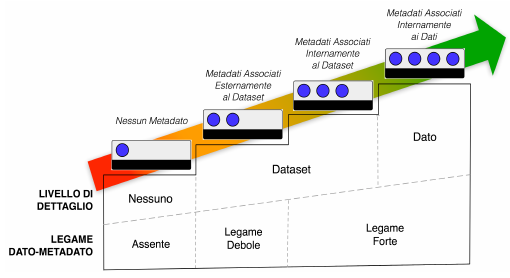
\includegraphics[width=250px]{metadati_classificazione.png} 
    %\caption{Modello di classificazione per i metadati.\footnote{Dalle \emph{Linee guida nazionali per il patrimonio informativo pubblico (2014)}.}  
  \end{figure}
\end{frame}

\section{5 Stelle}

\begin{frame}
  \frametitle{Classificazione 5 Stelle}

  Il w3c propone un modello per la qualit\`a degli open data denominato
  \emph{classificazione a 5 stelle}.\footnote{\url{http://5stardata.info}}
  Riportiamo il diagramma della classificazione 5 stelle riportato nelle linee
  guida dall'Agid.
  \vspace{\baselineskip}  
  
  \begin{figure}
     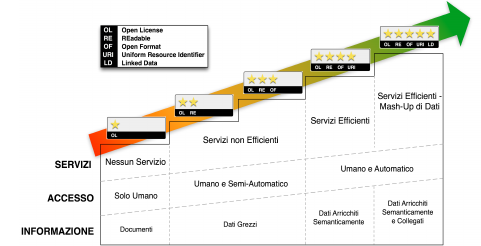
\includegraphics[width=300px]{5stelle_classificazione.png} 
    %\caption{Modello di classificazione per i metadati.\footnote{Dalle \emph{Linee guida nazionali per il patrimonio informativo pubblico (2014)}.}  
  \end{figure}
\end{frame}

\begin{frame}
  \frametitle{Classificazione 5 Stelle - Dimensioni}
  La classificazione 5 stelle viene estesa dall'AgID con alcune \emph{dimensioni}
  esplicative:
  \begin{itemize}[<+->]
   \item \emph{INFORMAZIONE} - descrive la qualit\`a dell'informazione fornita insieme ai dati;
   \item \emph{ACCESSO} -  descrive la facilit\`a con cui utenti e programmi riescono ad accedere ai dati;
   \item \emph{SERVIZI} - riguarda le tipologie e l'\emph{efficienza} dei servizi che possono essere realizzati a partire 
   dai dati.
  \end{itemize}
\end{frame}

  
\begin{frame}
  \frametitle{Classificazione 5 Stelle - Una Stella}
  
  Una Stella: Open Licence
  
  \begin{figure}
     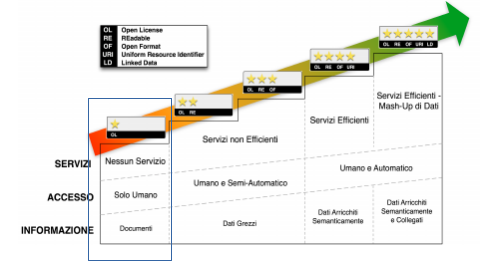
\includegraphics[width=180px]{stella1.png} 
    %\caption{Modello di classificazione per i metadati.\footnote{Dalle \emph{Linee guida nazionali per il patrimonio informativo pubblico (2014)}.}  
  \end{figure}
  
  La \emph{prima stella} si ottiene rilasciando i dati in qualunque formato
  ma con una \emph{licenza aperta}.
  Rientrano in questa categoria ad esempio le scansioni dei documenti.
  \vspace{\baselineskip}

  \begin{itemize}[<+->]
   \item \emph{INFORMAZIONE: documenti} - i dati sono incorporati all’interno di documenti senza struttura;
   \item \emph{ACCESSO: solo umano} - solo gli umani sono in grado di leggere i documenti senza struttura 
   e quindi dare un senso ai dati in esso presenti;
   \item \emph{SERVIZI: nessuno} può essere abilitato a meno di significativi interventi umani 
   di estrazione ed elaborazione;
  \end{itemize}
\end{frame}

\begin{frame}
  \frametitle{Classificazione 5 Stelle - Due Stelle}
  
    Due Stelle: Open Licence, (Machine) Readable

  \begin{figure}
     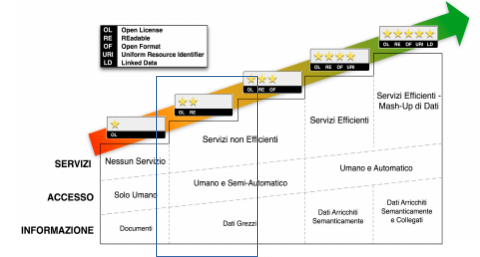
\includegraphics[width=180px]{stella2.png} 
    %\caption{Modello di classificazione per i metadati.\footnote{Dalle \emph{Linee guida nazionali per il patrimonio informativo pubblico (2014)}.}  
  \end{figure}
  
  La \emph{seconda stella} si ottiene se i dati sono forniti in un formato leggibile 
  da un agente automatico. 
  
  Rientrano in questa categoria ad esempio i files in formato \emph{excel}.
  \vspace{\baselineskip}

  \begin{itemize}[<+->]
   \item \emph{INFORMAZIONE: dati grezzi (o semi-strutturati)} - i dati sono leggibili anche da un programma 
   ma necessita un intervento umano per interpretarli;
   \item \emph{ACCESSO: umano e semi-automatico} - i software possono leggere i dati ma non sono in grado di
   interpretarli automaticamente;
   \item \emph{SERVIZI: non efficienti} - servizi realizzati ad-hoc e devono incorporare al loro
  interno i dati;
  \end{itemize}
\end{frame}

\begin{frame}
  \frametitle{Classificazione 5 Stelle - Tre Stelle}
  
  Tre Stelle: Open Licence, (Machine) Readable, Open Format

  \begin{figure}
     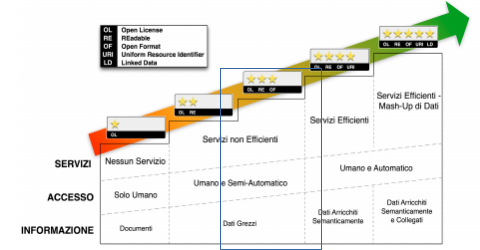
\includegraphics[width=180px]{stella3.png} 
    %\caption{Modello di classificazione per i metadati.\footnote{Dalle \emph{Linee guida nazionali per il patrimonio informativo pubblico (2014)}.}  
  \end{figure}
  
  La \emph{terza stella} viene attribuita se i dati sono rilasciati in un formato \emph{aperto}.
  Rientrano in questa categoria ad esempio i files \emph{jsono}, \emph{csv}, \emph{xml}.
  \vspace{\baselineskip}

  \begin{itemize}
   \item \emph{INFORMAZIONE: dati grezzi (o semi-strutturati)} - i dati sono leggibili anche da un programma 
   ma necessita un intervento umano per interpretarli;
   \item \emph{ACCESSO: umano e semi-automatico} - i software possono leggere i dati ma non sono in grado di
   interpretarli automaticamente;
   \item \emph{SERVIZI: non efficienti} - servizi realizzati ad-hoc e devono incorporare al loro
  interno i dati;
  \end{itemize}
\end{frame}

\begin{frame}
  \frametitle{Classificazione 5 Stelle - Quattro Stelle}
  
  Quattro Stelle: Open Licence, (Machine) Readable, Open Format, URI

  \begin{figure}
     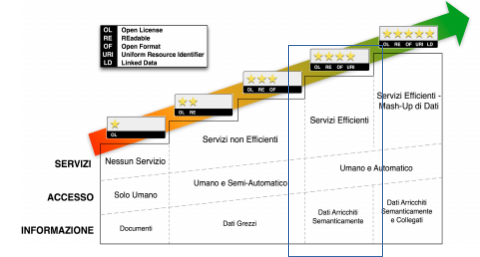
\includegraphics[width=180px]{stella4.png} 
    %\caption{Modello di classificazione per i metadati.\footnote{Dalle \emph{Linee guida nazionali per il patrimonio informativo pubblico (2014)}.}  
  \end{figure}
  
  La \emph{quarta stella} si ottiene esponendo i dati con le tecnologie del web semantico (RDF e SPARQL).
  \vspace{\baselineskip}

  \begin{itemize}[<+->]
   \item \emph{INFORMAZIONE: dati arricchiti semanticamente} - i dati sono descritti usando tecnologie del Web Semantico;
   \item \emph{ACCESSO: umano e automatico} - i software sono in grado di elaborare i dati quasi senza ulteriori 
   interventi umani (livelli 4 e 5);
   \item \emph{SERVIZI: efficienti} - servizi che sfruttano accessi diretti a Web per reperire i dati.
  \end{itemize}
\end{frame}

\begin{frame}
  \frametitle{Classificazione 5 Stelle - Cinque Stelle}
  
  Cinque Stelle: Open Licence, (Machine) Readable, Open Format, URI, \emph{Linked} Data

  \begin{figure}
     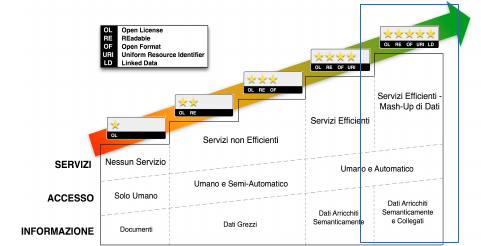
\includegraphics[width=180px]{stella5.png} 
    %\caption{Modello di classificazione per i metadati.\footnote{Dalle \emph{Linee guida nazionali per il patrimonio informativo pubblico (2014)}.}  
  \end{figure}
  
  La \emph{quinta stella} viene attribuita quando i dati contengono riferimenti a dataset di terze parti.
  \vspace{\baselineskip}

  \begin{itemize}[<+->]
   \item \emph{INFORMAZIONE: dati arricchiti semanticamente} - i dati sono descritti usando tecnologie del Web Semantico;
   \item \emph{ACCESSO: umano e automatico} - i software sono in grado di elaborare i dati quasi senza ulteriori 
   interventi umani (livelli 4 e 5);
   \item \emph{SERVIZI: efficienti e con mashup di dati} - servizi che sfruttano sia accessi diretti a Web 
   sia l'informazione ulteriore catturata attraverso i \emph{link} dei dati di interesse.
  \end{itemize}
\end{frame}

\end{document}
